\subsection{Density} 
\label{eos-density}

In subsurface oil and gas reservoirs, properties of gases and liquids strongly depend from environmental pressure and temperature conditions. Equations of state (EOS) may be used to describe the relationship of volume, pressure and temperature of a real fluid. The knowledge of a fluids volume or its density is essential to estimate further thermodynamic properties. The first EOS for real gases, which was based on the ideal gas law, was presented by Johannes Diderik {van der Waals} in 1873 \cite{VanWaa:73}. In 1910 he received the Nobel prize for the development of the equation
%
\begin{equation}
p=\frac{RT}{V_m-b}-\frac{a}{V^2_m}
\label{eq-van-der-waals}
\end{equation}
%
where $p$ is the pressure, $R$ is the gas constant, $T$ is the temperature, $V_m$ is the molare volume and $a$ and $b$ are correcting parameters. 

%---
\paragraph{Redlich-Kwong equation of state (RKEOS)}

The equation of {Redlich} and {Kwong} from 1949 \eqref{eq-rkeos1} represents just a little improvement of the van der Waals equation \cite{RedKwo:49}. It is given as
%
\begin{equation}
p=\frac{RT}{V_m-b}-\frac{a}{T^{0.5}\,V_m\,(V_m+b)}.
\label{eq-rkeos1}
\end{equation}
%
The results are satisfactory only for temperatures above the critical point (see Tab.~\ref{tab-eos2}). 

\begin{table}[H]
  \caption{\label{tab-eos2}Fluid properties used in equations of state, where $\omega$ is the acentric factor, $T_c$ and $p_c$ are temperature und pressure at the critical point and $R$ ist the gas constant.}
  \begin{center}
\begin{tabular}{lrrrr}
\toprule
  Fluid 		& $\omega$ [-]  & $T_c$ [K] & $p_c$ [MPa] & $R$ [J/kg/K]\\
\midrule
  Carbon dioxide & 0.239  			& 304.13 & 7.38 		& 188.9\\
  Ethane         & 0.099  			& 305.32	& 4.87 		& 276.5\\
  Methane        & 0.011  			& 190.56 & 4.60 		& 518.3\\
  Water          & 0.344  			& 647.10 & 22.06 		& 461.5\\
\bottomrule
\end{tabular}
\end{center}
\end{table}

Equation \eqref{eq-rkeos1} can be recasted as a cubic equation in terms of volume
%
\begin{equation}
V_m^3-\frac{RT}{p}V_m^2-\left(\frac{RTb}{p}-\frac{a}{T^{0.5}p}+b^2\right)V_m-\frac{ab}{T^{0.5}p}=0.
\label{eq-rkeos2}
\end{equation}
              
This equation yields to one or three real roots depending on the number of phases in the system. In the two-phase region, the largest positive root represents the molar volume of the gas phase while the smallest root correspondes to the volume of the liquid phase. The correcting terms $a$ and $b$ are given as
%
\begin{equation}
a=0.4275\,\frac{R^2 T_c^{2.5}}{p_c}
\label{eq-rkeos_a}
\end{equation}
%
and
%
\begin{equation}
b= 0.0866\,\frac{RT_c}{p_c}
\label{eq-rkeos_b}
\end{equation}
%
where $T_c$ and $p_c$ are Temperature and pressure at the critical point (see Tab.~\ref{tab-eos2}). Figs.~\ref{fig-eos-dens-ch4-co2} and \ref{fig-eos-dens-h2o-n2} show the results of the RKEOS for several substances at four different temperatures in comparison to other equations of state.

\begin{figure}
\subfigure[]{\label{fig-eos-dens-ch4}\includegraphics[width=0.5\textwidth]{figures/dens-ch4.eps}}
\hfill
\subfigure[]{\label{fig-eos-dens-co2}\includegraphics[width=0.5\textwidth]{figures/dens-co2.eps}}
\caption[]{\label{fig-eos-dens-ch4-co2}Density of \ch4~\subref{fig-eos-dens-ch4} and \co2~\subref{fig-eos-dens-co2} derived by different EOS. There stand 
\setlength{\unitlength}{1ex}
\begin{picture}(5,1)
\thicklines \put(0,0.5){\line(1,0){5}}
\end{picture}
for the \textsc{Helmholtz} Free Energy,
\begin{picture}(5,1)
\thicklines \multiput(0,0.5)(2,0){3}{\line(1,0){1}}
\end{picture}
for the PREOS and
\begin{picture}(5,1)
\thicklines \multiput(0,0.5)(2,0){3}{\line(1,0){1}}\multiput(1.4,0.5)(2,0){2}{\line(1,0){0.25}}
\end{picture}
for the RKEOS. The colours refer to different temperatures (\textcolor{blue}{blue} - $\unit[280]{K}$, \textcolor{violet}{violet} - $\unit[320]{K}$, \textcolor{purple}{pink} - $\unit[400]{K}$, \textcolor{red}{red} - $\unit[680]{K}$).}
\end{figure}

\begin{figure}
\subfigure[]{\label{fig-eos-dens-h2o}\includegraphics[width=0.5\textwidth]{figures/dens-h2o.eps}}
\hfill
\subfigure[]{\label{fig-eos-dens-n2}\includegraphics[width=0.5\textwidth]{figures/dens-n2.eps}}
\caption[]{\label{fig-eos-dens-h2o-n2}Density of \h2o~\subref{fig-eos-dens-h2o} and \n2~\subref{fig-eos-dens-n2} derived by different EOS. There stand 
\setlength{\unitlength}{1ex}
\begin{picture}(5,1)
\thicklines \put(0,0.5){\line(1,0){5}}
\end{picture}
for the \textsc{Helmholtz} Free Energy,
\begin{picture}(5,1)
\thicklines \multiput(0,0.5)(2,0){3}{\line(1,0){1}}
\end{picture}
for the PREOS and
\begin{picture}(5,1)
\thicklines \multiput(0,0.5)(2,0){3}{\line(1,0){1}}\multiput(1.4,0.5)(2,0){2}{\line(1,0){0.25}}
\end{picture}
for the RKEOS. The colours refer to different temperatures (\textcolor{blue}{blue} - $\unit[280]{K}$, \textcolor{violet}{violet} - $\unit[320]{K}$, \textcolor{purple}{pink} - $\unit[400]{K}$, \textcolor{red}{red} - $\unit[680]{K}$).}
\end{figure}

%---
\paragraph{Peng-Robinson equation of state (PREOS)}

D.\,Y.\,{Peng} and D.\,B.\,{Robinson} presented an improvement of the RKEOS in 1975 \cite{PenRob:75}. The proposed equation is also a two-constant van der Waals-Type equation and combines simplicity and accuracy. The PREOS is very simple to solve and gives satisfying results within the whole fluid redion of a gas. It is given in the form
%
\begin{equation}
p=\frac{RT}{V_m-b}-\frac{a(T_c)\cdot \alpha (T_r,\omega)}{V_m^2+2\cdot bV_m-b^2}
\label{eq-preos1}
\end{equation}
%
where $a$ and $b$ are correcting terms. They can be derived by %\eqref{eq-preosa} and \eqref{eq-preosb} 
%
\begin{equation} 
a(T_c) = 0.45724\,\frac{R^2T_{c}^{2}}{p_c}
\label{eq-preosa}
\end{equation}
%
and
%
\begin{equation} 
b(T_c) = 0.07780\,\frac{RT_c}{p_c}
\label{eq-preosb}
\end{equation}
%
for the particular fluids under specification of pressure and temperature at the critical point.
Parameter $\alpha(T_r,\omega)$ is a dimensionless function of reduced temperature $T_r$ and acentric factor $\omega$. It is given as
%
\begin{equation} 
\alpha = \left( 1+ \left(0.37464 + 1.54226\,\omega - 0.26992\,\omega^2\right)\left(1-T_r^{0.5}\right)\right)^2
\label{eq-preosalpha1}
\end{equation}
%
for $\omega\leq{0.49}$ and
%
\begin{equation} 
\alpha = \left( 1+ \left(0.379642 + \left(1.48503-\left(1.164423-1.016666\,\omega\right)\omega\right)\omega\right)\left(1-T_r^{0.5}\right)\right)^2
\label{eq-preosalpha2}
\end{equation}
%
for $\omega > 0.49$. 
%
Tab.~\ref{tab-eos2} shows acentric factors and critical parameters for different real gases. The resulting density distribution of the 
PREOS is shown in Figs.~\ref{fig-eos-dens-ch4-co2} and \ref{fig-eos-dens-h2o-n2} at four different temperatures. 

%---
\paragraph {Fundamental equations}			
For highly precise results it is necessary to adapt fundamental equations based on the free energy. The \textsc{Helmholtz} free energy is given as
%
\begin{equation}
\frac{f(\rho,T)}{RT}=\phi(\delta,\tau)=\phi^{o}(\delta,\tau)+\phi^{r}(\delta,\tau)
\label{eq-fhe1}
\end{equation}
in dependence from density $\rho$ and temperature $T$ in its dimensionless form. These dimensionless parts are given as the terms $\delta=\rho/\rho_c$ and $\tau=T_c/T$, whereas $\rho_c$ and $T_c$ are density and temperature at the critical point (see Tab.~\ref{tab-eos2}).  The \textsc{Helmholtz} free energy provides relations between density, temperature and all thermodynamic properties of a fluid, which are expressed in the parameter $\phi^{o}$ as the ideal gas part and $\phi^{r}$ as the residual part. For their derivatives in the short forms like
$\phi^r_\delta$,\hspace{0.1cm} 
$\phi^r_{\delta\delta}$,\hspace{0.1cm} 
$\phi^r_\tau$,\hspace{0.1cm} 
$\phi^r_{\tau\tau}$,\hspace{0.1cm} 
$\phi^r_{\delta\tau}$,\hspace{0.1cm}
$\phi^o_\tau$,\hspace{0.1cm} 
$\phi^o_{\tau\tau}$
it is refered to \cite{SpaWag:96}.

Everal authors used the approach of \textsc{Helmholtz} free energy to develop EOS for different substances, e.\,g.\,:
%
\begin{itemize}
\item {Span \& Wagner} \cite{SpaWag:96}, \cite{Spa:93}, \cite{SpaLem:00} for carbon dioxide and for nitrogen,
\vspace{-2mm}
\item {Pruss \& Wagner} \cite{PruWag:95}, \cite{WagPru:02} for water,
\vspace{-2mm}
\item {B\"ucker \& Wagner} \cite{BueWag:06} for ethane and
\vspace{-2mm}
\item {Setzmann \& Wagner} \cite{SetWag:91} for methane.
\end{itemize}

The fundamental equation (\ref{eq-fhe1}) according to {Wagner} et al.\ (\cite{SpaWag:96},\cite{PruWag:95},\cite{BueWag:06}, and \cite{SetWag:91}) is one of the most precise EOS at present. The equation and its derivatives can be used to describe all thermodynamic properties of a pure substance depending on density and temperature. So it is necessary to solve the relationship between density, pressure and temperature iteratively, as \eqref{eq-fhe-dens} shows
%
\begin{equation}
\frac{p(\delta,\tau)}{\rho RT}=1+\delta \frac{\partial \phi^r}{\partial \delta}.
\label{eq-fhe-dens}
\end{equation}

For water, the equation became international standard for the IAPWS\,\footnote{International Association for the Properties of Water and Steam} since 1995. Certainly, the equation is complicated to solve and requires long computing time. Therefore, several codes it is possible to choose between an iterative solving algorithm 
and an interpolation of density values out of a database. 

The semi-empirical fundamental equation \eqref{eq-fhe1} has to be fitted to measurement data by computer algorithms for each substance. Depending on the fluid, there are up to 200 adjusting coefficients to ensure a very accurate fit to the real gas behaviour. For each 
substance, equation \eqref{eq-fhe1} has separate ranges of validity, which are shown in Tab.~\ref{tab-eos-val}.

\begin{table}[H]
  \caption{\label{tab-eos-val}Ranges of validity of the free \textsc{Helmholtz} equation \eqref{eq-fhe1} for serveral fluids valid from the melting point up to the indicated 
  values.}
 \begin{center}
 \begin{tabular}{lrrl}
  \toprule
  	Fluid		&$T$ [K]    &$p$ [MPa]	& Reference\\
  \midrule
  Carbon dioxide 	& 216 		& 1100 		& \cite{SpaWag:96}, \cite{Spa:93}\\
  Nitrogen      	 & 1000 		& 2200 		& \cite{SpaLem:00}\\
  Ethane        	 & 520 		& 30 			& \cite{BueWag:06}\\ 
  Methane       	 & 625 		& 1000 		& \cite{SetWag:91}\\
  Water         	 & 1273 		& 1000 		& \cite{PruWag:95}, \cite{WagPru:02}\\
 \bottomrule
 \end{tabular}
 \end{center}
\end{table}

% The \textsc{Helmholtz} free energy provides relations between density, temperature and all thermodynamic properties of a fluid. Some of them are shown here: 
%
%$\phi^r_\delta = \left[\frac{\partial\phi^r}{\partial\delta}\right]_\tau$, $\phi^r_\delta\delta = \left[\frac{\partial^2\phi^r}{\partial\delta^2}\right]_\tau$, 
%$\phi^r_\tau = \left[\frac{\partial\phi^r}{\partial\tau}\right]_\delta$, $\phi^r_\tau\tau = \left[\frac{\partial^2\phi^r}{\partial\tau^2}\right]_\delta$, 
%$\phi^r_\delta\tau = \left[\frac{\partial^2\phi^r}{\partial\delta\partial\tau}\right]$, $\phi^o_\tau = \left[\frac{\partial\phi^o}{\partial\tau}\right]_\delta$, 
%$\phi^o_\tau\tau = \left[\frac{\partial^2\phi^o}{\partial\tau^2}\right]_\delta$.

%#####################################################################################################################
\subsection{Enthalpy}

The specific enthalpy $h$ is the whole amount of energy of a fluid. It consists of the internal energy and the volume changing work. It can be expressed by deviations of the free \textsc{Helmholtz} energy as
%
\begin{equation}
\frac{h(\delta,\tau)}{RT}=1+\tau\left(\phi^o_\tau+\phi^r_\tau\right)+\delta\phi^r_\delta.
\label{eq-fhe-enthalpy}
\end{equation}

%---
\subsection{Entropy}

The entropy $s$ represents which plenty of the energy of a system is potentially available to do work and which plenty of it is potentially defined as heat. In classical thermodynamics, the validity for the entropy is the thermodynamical system in equilibrium. The following equation is given for the entropy:
%
\begin{equation}
\frac{s(\delta,\tau)}{R}=\tau\left(\phi^o_\tau+\phi^r_\tau\right)-\phi^o-\phi^r.
\label{eq-fhe-entropy}
\end{equation}

%---
\subsection{Heat capacity}

The specific heat capacity of a fluid is defined as the amount of heat which is needed to increase the temperature of a fluid of $\unit[1]{kg}$ by $\unit[1]{K}$. In thermodynamics, it is distinguished between a heat capacity at constant pressure, the isobaric heat capacity, and a heat capacity at constant volume, the isochoric heat capacity. Both can be expressed in terms of free \textsc{Helmholtz} energy, like the following equations show:
%
\begin{itemize}
%
\item[]isobaric heat capacity
\begin{equation}
\frac{c_p(\delta,\tau)}{R}=-\tau^2\left(\phi^o_{\tau\tau}+\phi^r_{\tau\tau}\right)+\frac{\left(1+\delta\phi^r_\delta-\delta\tau\phi^r_{\delta\tau}\right)^2}{\left(1+2\delta\phi^r_\delta+\delta^2\phi^r_{\delta\delta}\right)} 
\label{eq-fhe-isobar}
\end{equation}
%
\item[]isochoric heat capacity
\begin{equation}
\frac{c_v(\delta,\tau)}{R}=-\tau^2\left(\phi^o_{\tau\tau}+\phi^r_{\tau\tau}\right).
\label{eq-fhe-isochor}
\end{equation}
\end{itemize}

\begin{figure}[t]
\subfigure[]{\label{fig-eos-enthalpy-co2}\includegraphics[width=0.5\textwidth]{figures/enthalpy-co2.eps}}
\hfill
\subfigure[]{\label{fig-eos-entropy-co2}\includegraphics[width=0.5\textwidth]{figures/entropy-co2.eps}}
\caption[]{\label{fig-eos-enthalpy-entropy-co2}Enthalpy~\subref{fig-eos-enthalpy-co2} and entropy~\subref{fig-eos-entropy-co2} of $\mathrm{CO_2}$ based on different EOS. There stand 
\setlength{\unitlength}{1ex}
\begin{picture}(5,1)
\thicklines \put(0,0.5){\line(1,0){5}}
\end{picture}
for the \textsc{Helmholtz} Free Energy,
\begin{picture}(5,1)
\thicklines \multiput(0,0.5)(2,0){3}{\line(1,0){1}}
\end{picture}
for the PREOS and
\begin{picture}(5,1)
\thicklines \multiput(0,0.5)(2,0){3}{\line(1,0){1}}\multiput(1.4,0.5)(2,0){2}{\line(1,0){0.25}}
\end{picture}
for the RKEOS. The colours refer to different temperatures (\textcolor{blue}{blue} - $\unit[280]{K}$, \textcolor{violet}{violet} - $\unit[320]{K}$, \textcolor{purple}{pink} - $\unit[400]{K}$, \textcolor{red}{red} - $\unit[680]{K}$).}
\end{figure}

\begin{figure}[htb]
\subfigure[]{\label{fig-eos-isobar-co2}\includegraphics[width=0.5\textwidth]{figures/isobar-co2.eps}}
\hfill
\subfigure[]{\label{fig-eos-isochor-co2}\includegraphics[width=0.5\textwidth]{figures/isochor-co2.eps}}
\caption[]{\label{fig-eos-isobar-isochor-co2}Isobaric heat capacity~\subref{fig-eos-isobar-co2} and isochoric heat capacity~\subref{fig-eos-isochor-co2} of $\mathrm{CO_2}$ based on different EOS. There stand 
\setlength{\unitlength}{1ex}
\begin{picture}(5,1)
\thicklines \put(0,0.5){\line(1,0){5}}
\end{picture}
for the \textsc{Helmholtz} Free Energy,
\begin{picture}(5,1)
\thicklines \multiput(0,0.5)(2,0){3}{\line(1,0){1}}
\end{picture}
for the PREOS and
\begin{picture}(5,1)
\thicklines \multiput(0,0.5)(2,0){3}{\line(1,0){1}}\multiput(1.4,0.5)(2,0){2}{\line(1,0){0.25}}
\end{picture}
for the RKEOS. The colours refer to different temperatures (\textcolor{blue}{blue} - $\unit[280]{K}$, \textcolor{violet}{violet} - $\unit[320]{K}$, \textcolor{purple}{pink} - $\unit[400]{K}$, \textcolor{red}{red} - $\unit[680]{K}$).}
\end{figure}

Due to the high number of adjusting coefficients, the properties based on the \textsc{Helmholtz} free energy may be seen as very 
accurate. On the other hand, the iterative solution of \eqref{eq-fhe-dens} takes long computing times, so for long-term simulations or for simulations with a high number of elements, it would be better to use the {van der Waals}-type equations of {Redlich-Kwong} or {Peng-Robinson}. These cubic equations are easy to solve and lead to results very fast. Figs.~\ref{fig-eos-enthalpy-entropy-co2} and \ref{fig-eos-isobar-isochor-co2} illustrate, in which range of temperature and pressure those simple EOS may be used. Here, thermodynamical properties of carbon dioxide based on temperature and density are shown calculated by different EOS. In general, if temperature rises while pressure is declining, the behaviour of a fluid approaches to that of the ideal gas and the cubic equations of state give suitable results. For instance, the resulting entropy and enthalpy values of carbon dioxide at low pressures and high temperatures are identical, regardless of the density model they are based on (see Fig.~\ref{fig-eos-enthalpy-co2} and \ref{fig-eos-entropy-co2}). In the liquid and the dense supercritical region, the results based on different EOS diverge increasingly.

In addition, in the vicinity of the saturation curve, the results based on the {van der Waals}-type EOS may show large variations compared to the fundamental equation based curves (\textsc{Helmholtz} free energy). Particularly, this becomes apparent from Figs.~\ref{fig-eos-isobar-co2} and \ref{fig-eos-isochor-co2}, where the heat capacities of $\mathrm{CO_2}$ are given. The heat capacities at $\unit[400]{K}$ and $\unit[680]{K}$ (in the supercritical region of $\mathrm{CO_2}$, where no phase boundary exists) are identical, independent from according density model. Within the two-phase region at $\unit[280]{K}$ and $\unit[320]{K}$, a strong deviation at the phase boundary can be seen.

For water, the cubic EOS are not suitable. Water is a high critical fluid, so its properties are to complex to be described by simple approaches. As we can see in Fig.~\ref{fig-eos-dens-h2o}, the RKEOS, as well as the PREOS equation give viable results only at pressures below $\unit[1]{MPa}$ and at high temperatures. Therefor it is recommended to use the fundamental equation of the \textsc{Helmholtz} free energy to estimate the density of water. 

